\section{Results and Discussion}\label{sec:results}

\subsection{Quantitative Results}
Table~\ref{tab:results} compares all models on 32 test images after decoding, with latent noise $\sigma=0.3$. The noisy input reaches an MSE of 0.00416, and the clean autoencoder output (0.00026) is the best any latent denoiser can reach. All denoisers improve on the noisy input. The MLP is the best denoiser on MSE, PSNR and SSIM. The four EPQD models are second and are close to each other, and EPQD-L is the best of them. The U-Net has the highest MSE of the denoisers, but it has the best FID, followed by the MLP. The EPQD models reduce the FID from 89.7 to about 70, which is worse than both classical baselines.

\begin{table}[t]
\centering
\caption{Image-level results on 32 test images (MSE, PSNR, SSIM) and FID on 1{,}000 test images. Best denoiser in bold.}
\label{tab:results}
\begin{tabular}{lcccc}
\toprule
\textbf{Model} & \textbf{MSE} & \textbf{PSNR (dB)} & \textbf{SSIM} & \textbf{FID}\\
\midrule
Conv-AE (clean) & 0.00026 & 35.85 & 0.989 & 9.0\\
Noisy latent & 0.00416 & 23.80 & 0.897 & 89.7\\
\midrule
MLP & \textbf{0.00245} & \textbf{26.12} & \textbf{0.931} & 58.4\\
U-Net & 0.00373 & 24.28 & 0.918 & \textbf{51.2}\\
EPQD-S (4q, 1 layer) & 0.00300 & 25.23 & 0.919 & 70.0\\
EPQD-M (4q, 2 layers) & 0.00298 & 25.26 & 0.920 & 70.0\\
EPQD-L (4q, 3 layers) & 0.00294 & 25.32 & 0.920 & 69.7\\
EPQD-IQP (4q, 2 layers) & 0.00301 & 25.22 & 0.919 & 70.1\\
EPQD-6Q-V2 & -- & -- & -- & --\\
\bottomrule
\end{tabular}
\end{table}

At patch level, the noisy input has an MSE of 0.0915. The EPQD models reduce it to 0.0313 (S), 0.0312 (M), 0.0308 (L) and 0.0314 (IQP), whereas the MLP reaches 0.0257. Patch-level and image-level values are measured in different spaces and should not be compared directly.

\subsection{Qualitative Results}
Figure~\ref{fig:qualitative} shows reconstructions of the same test images for the original, the noisy latent, the baselines and the EPQD models.

\begin{figure*}[t]
\centering
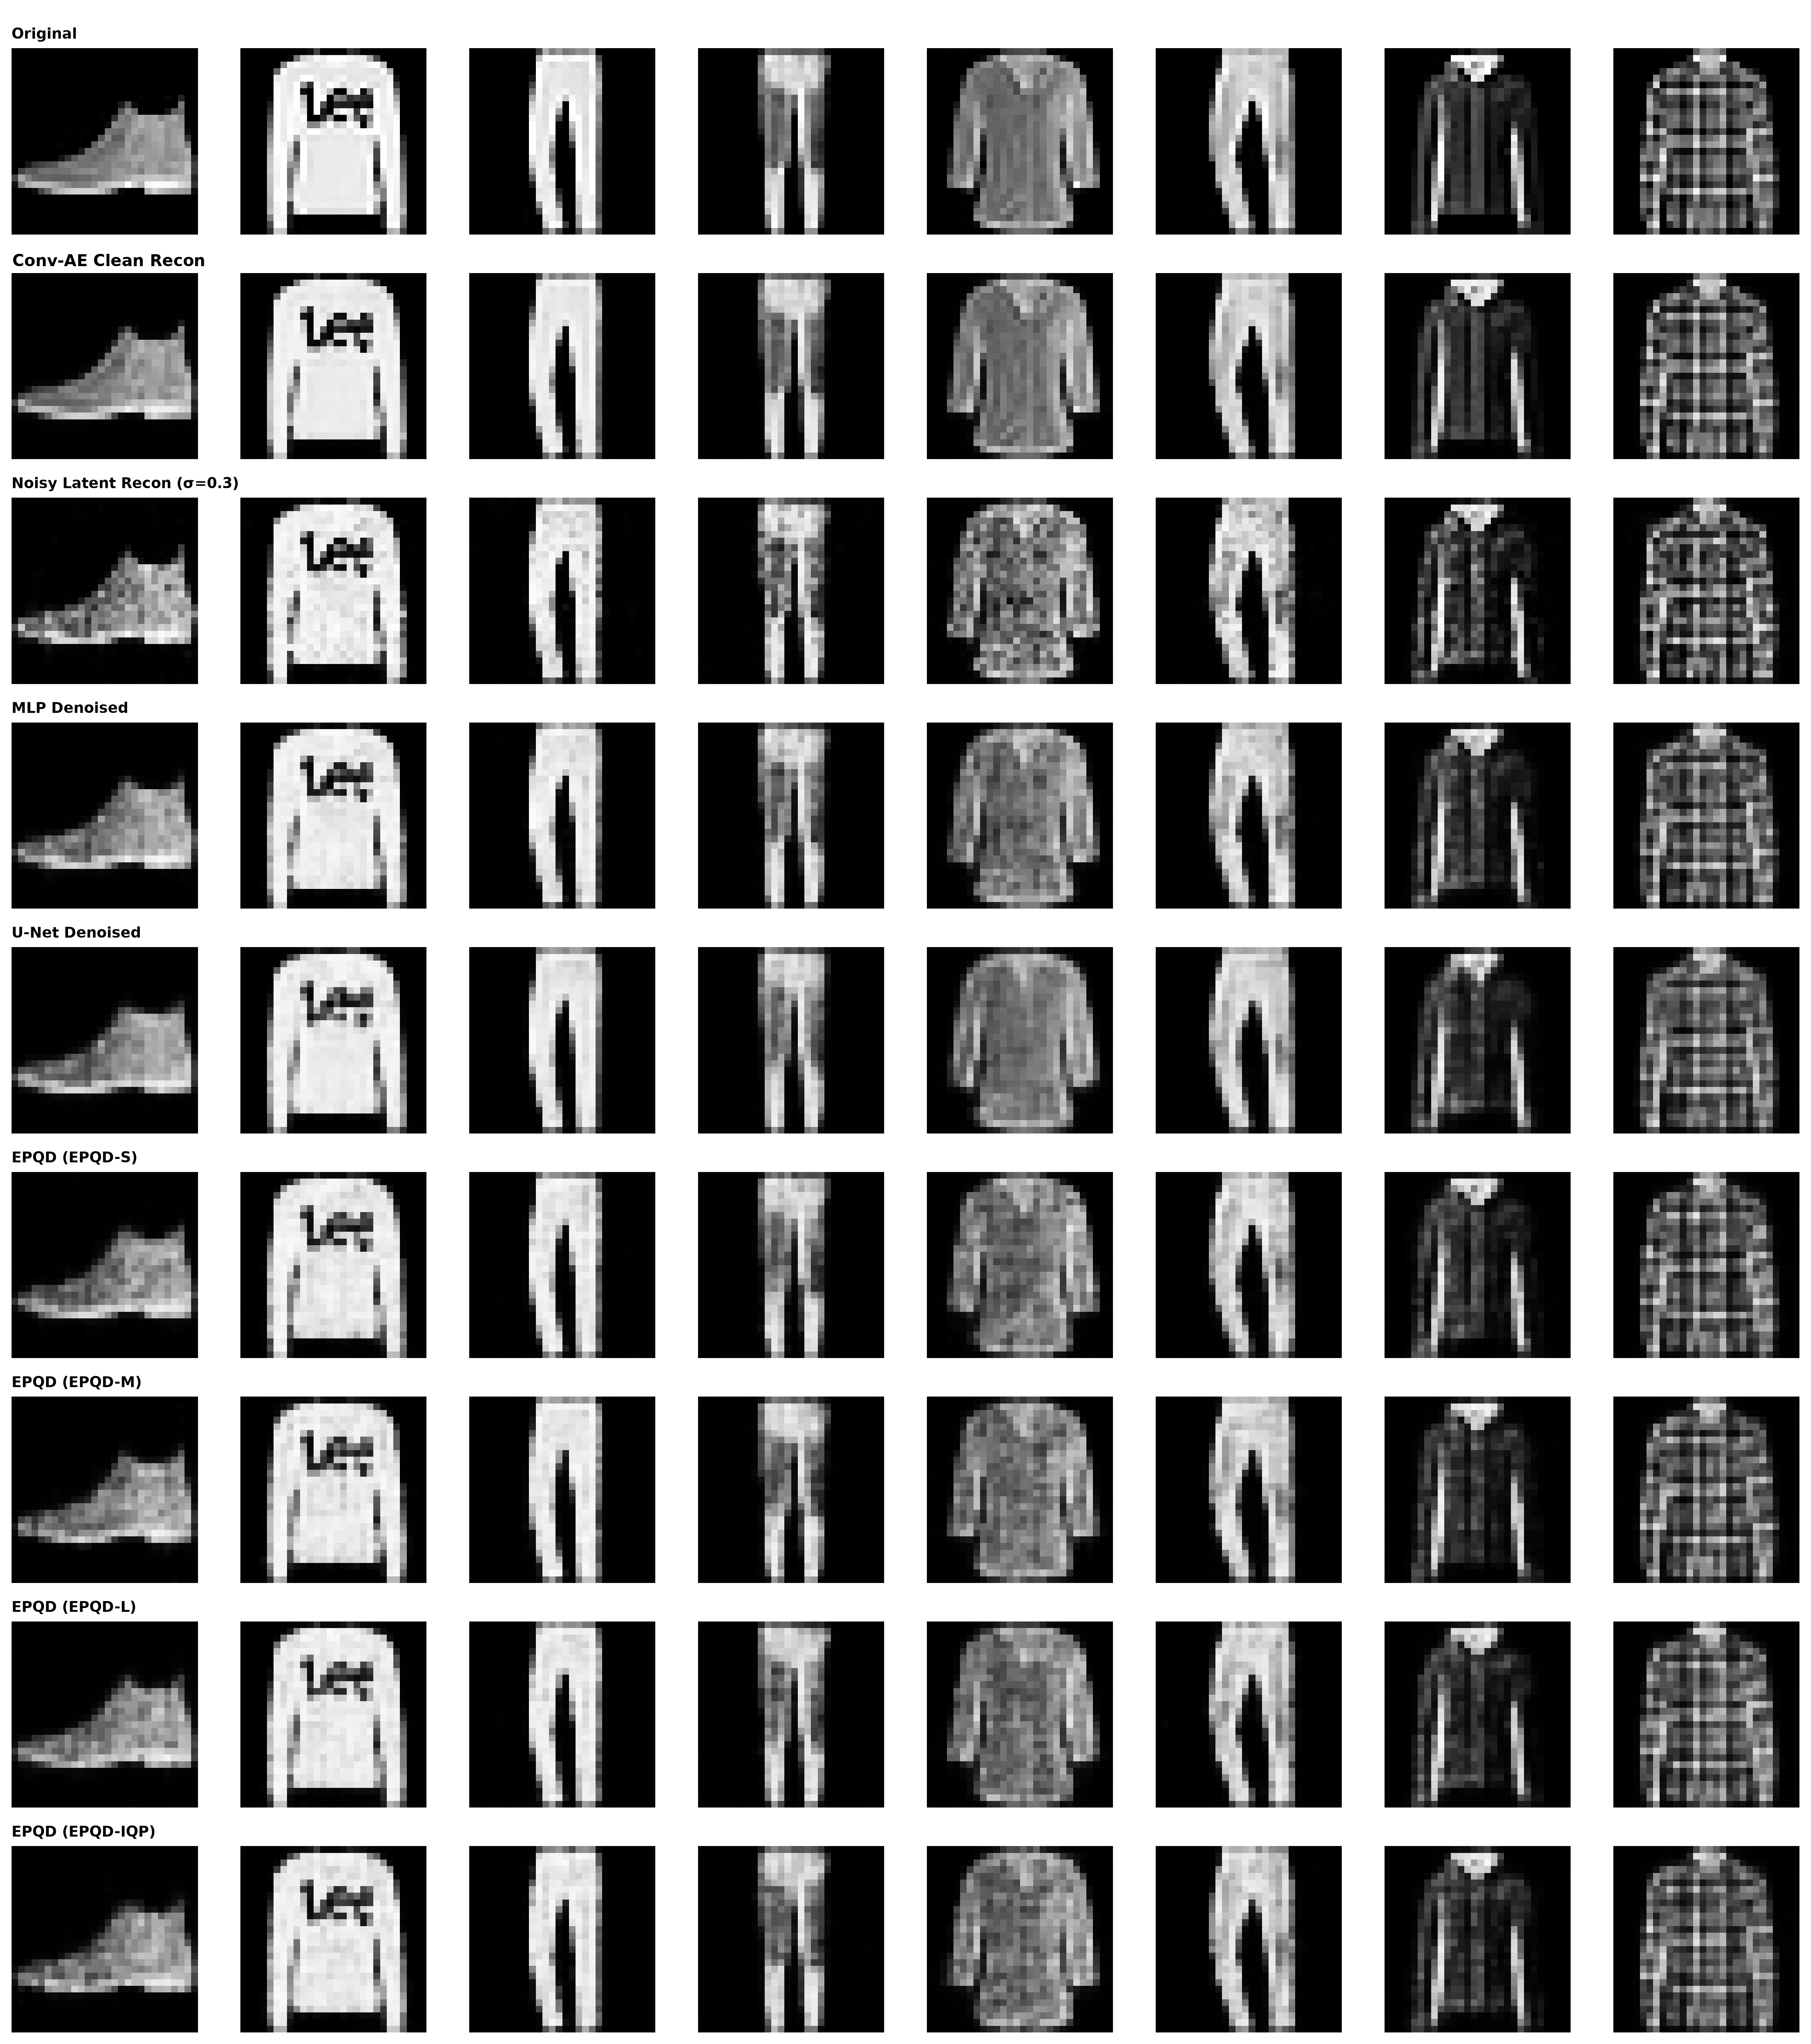
\includegraphics[width=0.72\textwidth]{PHQD_full_comparison.png}
\caption{Reconstructions of the original image, the noisy latent, the classical baselines and the EPQD variants.}
\label{fig:qualitative}
\end{figure*}

\subsection{Discussion}
Deeper circuits help only slightly: going from one to three layers lowers the image MSE from 0.00300 to 0.00294. The IQP-style encoding is not better than the basic ring circuit with the same depth (0.00301 against 0.00298). Each model was trained once, so these small gaps cannot be called significant. The main result is that the best classical baseline, the MLP, beats every 4-qubit hybrid model, which agrees with the finding of Bowles et al.~\cite{bowles} that strong classical models are hard to beat. This is also why classical baselines and ablations are needed before crediting the circuit. EPQD-6Q-V2 changes several things at once (qubit count, repeated encoding, three measurement bases, wider projections, joint stitching fine-tuning and an SSIM loss), so any gain over the 4-qubit models cannot be assigned to the qubit count alone.

\subsection{Computational Cost}
All circuits are simulated on the classical \texttt{default.qubit} simulator with batched evaluation and backpropagation, which avoids one circuit call per patch. No physical quantum hardware was used. The wall-clock times and memory use are [fill in from your logs].
